
\newrefsection

%\textbf{B1.a. Extended Synopsis of the scientific proposal}

\chapter{B1.a. Extended Synopsis of the scientific proposal}\label{part1}

\eu{(max 5 pages)}

\eu{The Extended Synopsis should give a concise presentation of the scientific
proposal, with particular attention to the ground-breaking nature of the
research project and the feasibility of the outlined scientific approach.
Describe the proposed work in the context of the state of the art of the field.
References to literature should also be included. References do not count
towards the page limits. It is important that this extended synopsis contains
all essential information including the feasibility of the scientific proposal
since the panel will only evaluate Part B1 at step 1.}

\section{Long-term vision and ground-breaking nature of the project}

The service and companion robots that we are set to interact with in the coming
years, are being designed and built today in labs and startups all over the
world. How can we ensure 'by design' that they will have a net social utility?
In other words: at the age of deep neural network and large language models,
what are the conditions for ensure responsible social robots?

\project will build the \textbf{new science required for robots to represent, reason and
act in complex social environments}, with the goal of realising \textbf{a vision
of social robots that enable humans and humans relationships to thrive}.
\project is about creating the conceptual and technical frameworks required for
safe and responsible social robots, intrinsically driven to foster stronger
social interactions with and between humans.

\textbf{\project main objective is, within 5
years, to design, implement and demonstrate in the real-world the AI engine of a
responsible socially intelligent robot}. Using the complex use-case of social
isolation in elderly care centres, we will show that a social robot that
implements Responsible Robotics principles, is accepted and adopted on the long
term by the stakeholders, and can have a genuinely positive, long lasting,
impact on the well being of older people.

This objective is underpinned by two research hypotheses: (\textbf{H1}) for
end-users to ascribe social utility and engage with the robot over long periods
of time (months, years), the robot has to have its own long-term internal
motivation to be socially helpful -- a \emph{social teleology}.

(\textbf{H2}) Additionally, long-term acceptance also requires the
genuine involvement of end-users in the shaping of the robot behaviours. As I
have shown in my past research, this user engagement generate trust, feeling of
ownership, and foster acceptance. Extrapolating from my laboratory result on
interactive machine learning, I hypothesise that this process may lead to
\emph{mutual accomodation} and eventually long term acceptance of a robot able
to continuously adapt to the need of its users.

To test and verify these two hypotheses in the real-world requires
\textbf{breaking new ground in science and engineering}. Critically, we need to
endow robots with a powerful way of representing and reasoning about their
social environment.  \project aims at achieving this breakthrough by developing
the mathematical models underpinning the recently discovered \emph{social
embeddings}, and significantly expanding their expressiveness.

\begin{framed}
\bf

\noindent My research vision is of socially-useful robots which
progressively learn to become autonomous, with the direct help and guidance
of their end-users. By doing so, the stakeholders actively shape the robots'
roles and behaviours, based on their actual, real-world needs and
experience, while ensuring ethical behaviours.

\noindent As such, my research program is about exploring, designing and
implementing novel methods for \emph{social learning} for assistive robots.
\emph{Social learning}, in this context, means developing machine learning
techniques using \emph{real world}, \emph{in-context} demonstrations by the
\emph{end-users themselves} to learn task and social action policies for the
robots.

\vspace{0.4em}


\noindent The envisioned outcome is not only assistive robots with a higher
degree of social autonomy, able to flexibly adapt, but also robots deeply
shaped and \emph{owned} by their users, and thus more readily accepted and adopted.

\vspace{0.4em}
Achieving this vision requires the combination of complex robotic socio-cognitive
capabilities, state-of-art machine learning techniques, and novel
experimental methodologies. Specifically my research will explore and enable:

\begin{itemize}
        \item compact, embedding-based representations of the social and spatial
            context of the robot;
        \item Attention-based deep machine learning architectures to learn
            context-appropriate behaviour sequences for social robots;        
        \item `end-user in-the-loop' data acquisition methodologies, including
            immersive teleoperation and progressive autonomy;
        \item the study of adoption barriers to such autonomous robots in
            human environments, with an initial focus on healthcare and elderly
            care.
\end{itemize}


\vspace{0.4em}
\noindent In addition, I will deliver the conceptual and ethical framework
required to further support the public debate and policy making process
around intelligent autonomous social robots, also through real-life demonstrations and
    deployments of assistive robots in high impact, complex social environments.

\vspace{0.4em}
\noindent Closely aligned with national and European research priorities,
this research program creates a excellent opportunity to reinforce INRIA and
Europe as worldwide leaders in Social and Intelligent Robotics.

\end{framed}


\subsection{Framing and research objectives}

AI and robots are emerging as key factors to successfully address modern societal
challenges, like the ageing society or increasing social isolation. In this context, how to
ensure \emph{by design} that social robots have a positive social impact?
This question is the backbone of my research project, and my research vision
is to \textbf{create within 5 to 10 years socially-intelligent and responsible robots,
that (1) will have recognised social utility, and (2) will see long-term
acceptance by their users}.
%
%I formulate two main hypotheses: (1) this objective can only be achieved if the
%robot is socially-driven: the robot's behaviours must be intrinsically driven
%by the intention to support positive human-human interactions (a \emph{social
%teleology}). How this general principle translates into specific guidelines and
%algorithms -- while taking into account the principles of a responsible AI --
%is a central research area of my project.

\vspace{0.4em}



%The overall aim of my research program is to \textbf{enable responsible,
%long-term social human-robot interactions}.
This translates into three overarching, long-term research questions:

\vspace{0.5em}
\begin{itemize}
    \item What are the public expectations with respect to the role of social
        robots, and how can we \textbf{collaboratively design}
        \textbf{autonomous}, yet \textbf{responsible, beneficial, socially
        acceptable robots}?

    \item What are the conceptual, algorithmic and technical prerequisites to
        design and implement such an autonomous \& responsible robots? in
        particular, what social context understanding and (machine) learning
        architectures are required to \textbf{enable long-term autonomy} and,
        eventually, \textbf{engagement} between a robot and its end-users?

    \item What are the conditions and methodologies enabling large scale data
        acquisition of \textbf{real world, user-driven robots behaviours}? How
        to then train robots to become \textbf{progressively autonomous}?  And
        ultimately, how to balance \textbf{autonomy} of the robot with the
        necessary \textbf{behaviour transparency} and \textbf{human oversight}?

\end{itemize}

\vspace{0.5em}
\noindent From these questions, I derive the following four objectives that are
the guiding principles of my research program, both in the short term, and at a
10-15 years horizon:

\subsection{Methodology}

Actual utility and long-term acceptance requires genuine involvement of the
end-users at every step of the design process. This is at odds with the common,
engineering-centered practise of first developing robots and algorithms \emph{ex-vivo}, in
lab, and then placing a (semi) final product in the hands of the users, hoping
for adoption. Adoption, however, is the result of a long process of \emph{mutual
modelling}~\autocite{sabanovicRobotsSocietySociety2010}, where
the social role of the robot is slowly constructed from its real world, in-context
usage.

This foundational insight requires the conceptual framing and development of new
research methodologies.  I have started to explore these questions in some of my
previous work~\autocite{senft2016sparc,winkle2019effective,winkle2021leador},
and my research program aims at significantly developing this line of research
to tackle more complex, long-term application domains.

One of the major challenge arising with more complex application domains is
however the combinatorial growth of the problem space. Indeed, none of the
current control paradigms or cognitive modelling techniques are able to
successfully predict context- and task-appropriate sequences of behaviours
for socially-useful autonomous robots.

\vspace{0.4em}

My research programme aims at tackling this challenge with two key insights: (1) the
representation complexity of the social and spatial environment of the robot 
can be dramatically reduced by treating it as an \emph{embedding} problem and
applying modern machine learning techniques (like GANs) to design and compute
\emph{social embeddings}; (2)
modern transformers and attention-based~\autocite{vaswani2017attention} machine learning
architectures have demonstrated long-term modelling
capabilities on complex language domains~\autocite{instructgpt2022} that could
in principle be equally applied to action sequence generation for
robots. Initial explorations of this second insight have started to
emerge~\autocite{rt12022,vemprala2023chatgpt}, but none of these early research
efforts consider the complexity of human interactions.

\vspace{0.4em}

My research program will research how these insights can be effectively
operationalized, with a scientifically ambitious
and highly technical work program. It includes basic research and conceptual
framing; extensive, beyond-state-of-art, technical developments; and an
ambitious experimental program, centered on long-term `user in-the-loop' data
collection via field deployments of social
robots in public spaces -- and primarily in the healthcare and elderly care
environment.


\subsection{Work plan outlook}

My research program could begin rapidly, using publicly available resources,
including machine learning architectures like Transformers, combined with open-source
pre-trained Large Language Model backbones; and state-of-art HRI tools like
ROS4HRI~\autocite{mohamed2021ros4hri} to represent in real-time the social
environment of the robot. While long and complex data collection campaigns would
have to be organised, and training infrastructure would need to
be designed, I expect initial results in the first 3 to 5 years.

This is also a long-term vision: on the one hand, the rapid pace of progress
of technology (novel deep machine learning architectures, novel HRI tools for
human and scene understanding) continuously opens novel investigation
venues; one the other hand, the success of my research vision hinges on
real-world, long-term experimental work: deploying robots in the healthcare
sector, creating the conditions for adoption by the end-users, running
long-term deployments with the end-users are long terms aims
,... these research activities will take
place over long period of time.

\subsection{Importance and impact}

My research program has the potential to be groundbreaking: until now,
autonomous social robots have had little real world success. Experiments and
deployments have been mostly limited to constrained application domains, where
rigid action policies (scripts, task planners) could be sufficient. State-of-art
robots however fail to handle the complexity and unpredictability of real world
environments (like the ones encountered in the healthcare domain). In addition,
these systems see poor field adoption due to several factors including
difficulty of use, wrong expectations, perceived complexity.

The novel paradigm that I will develop and deploy as a Directeur de
Recherche at INRIA addresses both this limitations. By using state-of-the-art
machine learning techniques -- with powerful abilities to adapt to unknown context
-- combined with a novel `user-in-the-loop' approach to data collection and
behaviour shaping, I believe we can overcome both challenges: real-world
autonomy, and adoption by the end-users.

This research program is also hugely important: as socially assistive robots quickly
develop, it is critical to equip ourselves with a deeper understanding and
intellectual framing of what social robots \emph{can} and \emph{should} be,
paving the way for their much broader adoption in the coming years: as a
Directeur de Recherche, I will actively contribute to this aim, by leading the
design and implementation of socially-intelligent robots that are socially
useful, acceptable in the long-term, and ethically responsible, but also by
furthering my engagement to interdisciplinary work, and broad engagement with
the society and policy makers.







%%%%%%%%%%%%%%%%%%%%%%%%%%%%%%%%%%%%%%%%%%%%%%%%%%%%%%%%%%%%%%%%%%%%%%%%%




%How this general
%principle translates into specific guidelines and algorithms -- while taking into
%account the principles of a responsible AI -- is the central
%contribution of Work Package 1.

% This socially-driven goal forms what we call a \emph{social
%teleology}. its own goals have this objective can only be achieved if the
%robot is \textbf{socially-driven}: the robot's behaviours must be driven by the
%intention to support positive human-human interactions. 


\project frames this hypotheses with the novel
idea of \textbf{robot-supported human-human interactions}, which reverses the
traditionally accepted, technology-centric, view on human-robot interactions.
Instead of having the robot at the centre of the stage, the humans are: we build
from pre-existing social interactions between people, and investigate where,
when and how robots could facilitate and enrich them. To this end, we will
deploy the \project robot for a year in a public space (the Bristol Science
museum, WeTheCurious), asking visitors to 'take control' of the robot for a
period of time, and use it to mediate interactions between other visitors of the
museum.  At the end of this experiment, we expect thousand of people to have had
experienced how robots could positively interact with humans, and each of these experiences
will contribute to uncovering and designing the basic principles of social interaction for
robots. This work is the focus of WP1.

While most of the interactions in the museum will be short-lived, two further
large scale experiments will take place over the course of the project: a
one-year experiment at the Bristol's children hospital, where the robot will
join one of the wards for children with long-term conditions, and engage the
children in playful social activities; another one-year experiment in one of
Bristol's Special Education Need (SEN) school, helping children with
psycho-social impairements to develop their social skills. In both these
experiments, the robot behaviours will be co-designed with, and learnt from the
end-users themselves: nurses, teachers, parents, and where possible, the
children themselves.


\begin{wrapfigure}{l}{0.2\linewidth}
    \centering
    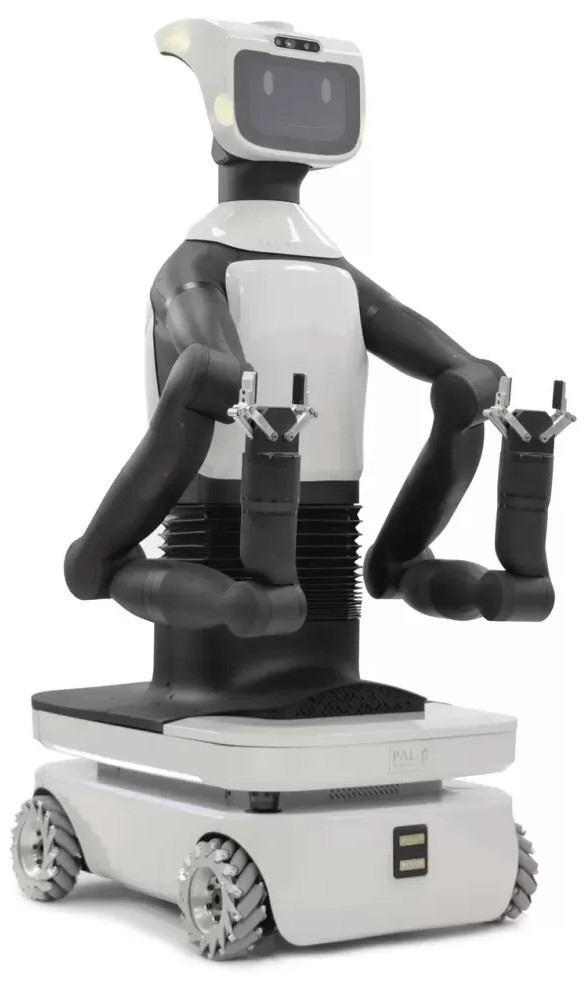
\includegraphics[width=\linewidth]{tiagopro}
    \label{fig|tiagopro}
\end{wrapfigure}

Importantly, \project focuses specifically on the AI engine of the robot: I will
use an existing robotic platform (PAL Robotics TIAGo Pro, pictured on the left) and develop and train the
algorithms required to achieve autonomy and responsible, long-term social utility. After the
initial training period, the robot will indeed be \emph{autonomous}: while the
users will be provided tools to override the robot decisions at any time (via
both an app and touch sensors on the robot itself), it will otherwise
move and act on its own, without the need for constant supervision. To this end,
the robot will have ground-breaking perception and modelling capabilities (the
focus of WP2) to represent the current social situation, coupled with an
innovative cognitive architecture designed to combine internal social
drives with domain-specific action policies learnt from the end-users (WP3).

The robot actions themselves are designed to be limited to non-verbal
communication mechanisms: non-verbal utterances using sounds, gaze, joint
attention, expressive motions. My team will in addition create a novel
non-verbal modality based on \emph{soundscapes}: sound landscapes that the robot
can modulate to influence the mood of the social environment (calm, excited,
worried, etc.) (WP4).

Finally, \project is also about asserting and reinforcing the European
leadership in AI and intelligent robotics, in line with EU strong societal
values: a socially responsible AI, that guarantees, by design, long-term
benefits to the society. This requires leading major technological advances;
leading the development of the conceptual framework around socially intelligent
robots that we need to inform future policy making; but also \textbf{a strong
leadership to meaningfully involve the public at large in the design of these
technologies}. Through its objectives and methodology, \textbf{\project will
have a major contribution to building this capacity in Europe}. 

\begin{framed}

\bf Over the 5 years of the fellowship, I will design and deliver a ground-breaking embodied AI for
socially intelligent robots, with long-term social utility and fully accepted in
the field.
    
This breakthrough is made possible by a combination of novel methodology and
complex integration:
\begin{itemize}
        \item crowd-sources social interaction patterns;
        \item `public-in-the-loop' machine learning;
        \item integration of the robot's disparate perceptions into a novel
            spatio-temporal and social situation model of the environment;
        \item novel, non-repetitive, social behaviour generation based on
            generative neural networks;
        \item and finally, an integrative cognitive architecture, driven by
            long-term social goals.
\end{itemize}

In addition, I will deliver the conceptual and ethical framework required to
further support the public debate and policy making process around social
robots, and concretely demonstrate lifescale applications of these robots in
two, one-year-long demonstrations in socially sensitive environments.

\end{framed}

\section{Feasibility of the \project work programme}

Socially intelligent robots require unique, beyond state-of-the-art,
capabilities to \emph{(1)} understand the social interactions (social
situation awareness), \emph{(2)} autonomously decide the best course of action for
short-term and longer-term social influence, and \emph{(3)} perform the
appropriate social actions and exert said influence in an appropriate,
responsible manner.
Not only the required technology is itself beyond state-of-the-art (and will be
researched and integrated in WP2, WP3 and WP4), but the
interplay between technology, socio-cognitive psychology, privacy and ethics is
only starting to be researched and understood. \project offers an
strong vision and an ambitious, evidenced-based, methodology to significantly
advance our understanding of this multi-faceted problem.

Over the course of 5 years, I will investigate hypotheses H1 and H2
by addressing the following research objectives:

\begin{itemize}
    \item \textbf{O1: conceptual framing} To construct a solid conceptual
        framing around the multidisciplinary question of responsible human-robot
        interactions, answering questions like: What should motivate the robot
        to step in and attempt to help? or: What social norms are applicable to
        the robot behaviours? Building on the extensive body of work on
        Responsible AI, I will investigate the basic principles of
        responsible robot-mediated social interactions, that must form the
        foundations of a socially useful robot, accepted and used in the long
        run.  Using user-centred design and participatory design methodologies,
        I will identify the determinants and parameters of a responsible social
        intervention, performed by a socially-driven robot, and formalise them
        in practical principles.

    \item \textbf{O2: physical-social representation and reasoning} To
        effectively and responsibly interact with its environment, the robot
        must first build a comprehensive and continously updated model, from its
        spatial and physical configuration, to its social dynamics. I will
        design and develop a novel cognitive capability of artificial
        \emph{social situation assessment} to enable the robot to represent
        real-time social dynamics in its environment. I will achieve this
        breakthrough by combining existing model-based approaches \TODO{refs}
        (including my recent research on social state modeling \TODO{refs}, with
        the expressive power of the new \emph{social embeddings} that I have
        recently introduced.

    \item {\bf O3: goal-driven, responsible decision making} I aim to create
        robot behaviours that are perceived as purposeful and intentional
        (long-term goals), while being shaped by a user-created and
        user-controlled action policy.  I will integrate long-term social goals,
        arising from the interaction principles of \textbf{O1}, with the social
        modeling capability of \textbf{O2}, into a principled, goal-driven
        cognitive architecture, with responsible AI guarantees. The breakthrough
        will come from combining these long-term social goals with bottom-up
        action policies, designed and learnt from the end-users using
        human-in-the-loop attention-based machine learning.

        I want to specifically test the following two hypotheses: first, that
        long-term social goals, if suitably co-designed with the public and
        stakeholders and properly integrated into the robot as a \emph{social
        teleology}, will create the perception that the robot is intentional and
        purposeful. This will in turn elicit sustained engagement from its human
        users.

        Second, that human-in-the-loop machine learning can be used to ensure an
        additional layer of human oversight and a level of behavioural
        transparency.  Human-in-the-loop reinforcement learning -- as
        implemented in the SPARC approach that I have developed with my students
        and already used in complex social
        environments~\parencite{senft2017supervised,senft2019teaching,winkle2020insitu}
        -- relies on an end-user `teacher'. This teacher initially fully
        controls the robot (via teleoperation) while it learns the action
        policy, and then progressively relinquishes control up to a point where
        the robot is effectively autonomous. As I previsouly argued
        in~\textcite{senft2019teaching}, this approach leads to increased
        control and ownership of the system, and as a result, increased trust
        from the end-users.


    \item{\bf O4: ambitious field research} Finally, the last major objective of
        my research project is to demonstrate the effectiveness of my approach
        in complex, real-world conditions. This means deploying the socially
        interactive robots in existing social \emph{ecosystems} that are
        sufficiently complex and open to explore novel social interactions. My
        objective is also to show that this real-world deployment can be
        successfully driven by the `end-to-end' involvement of all the end-users
        and stakeholders: from defining the robot's role, from the different
        perspective of each end-user, to actually designing and `teaching' the
        robot what to do.


\end{itemize}


These objectives are investigated across five work-packages: \textbf{WP1}
is dedicated to the conceptual framing of the project (O1); \textbf{WP2} builds
on the principles identified in WP1, and translates them into socio-cognitive
representations and capabilities, identifying and filling the gaps in the
state-of-the-art (O3); in parallel to WP2, \textbf{WP3} transposes the
conceptual framework of WP1 into a principled cognitive architecture and
integrates together the cognitive functions of WP2 (O2); \textbf{WP4} looks at
how social robots can perform effective social interventions to exert positive
social influence (O3); and \textbf{WP5} organises the experimental fieldwork
that demonstrates the \project approach in ambitious and
complementary real-world situations (O4).

\subsection{WP1: \textbf{\wpOne}}

WP1 aims at establishing the conceptual framework around the idea of
\emph{robot-supported human-human interactions}. It does so by co-creating
modes of interaction and norms with the general public, using a unique
combination of ethnographic observations and `public-in-the-loop' machine
learning.

\begin{framed}
    \textbf{Main outcomes:} A theoretical framework
to `think' the role of social robots and inform policy making (including ethical implications); a set
of operational \& co-created interaction principles; a large dataset of social
human-robot interactions

    \textbf{Duration:} \textbf{Y1-Y3}; one senior post-doc
with background in sociology of technology.
\end{framed}


\textbf{T1.1 -- Conceptual framing and ethics of robot-supported social
interactions}


The first task in WP1 is to research and define the framework that will provide the (currently missing) conceptual
frame around questions like: what role for social robots? where to set the
boundaries of artificial social interactions? what does 'ethical-by-design',
'responsible-by-design' might mean in the context of social human-robot
interactions? 


This first task is a pre-requisite for each of the field experiments (T1.1,
T5.1. T5.2), and will cover the whole duration of the project. This work is
coordinated by the PI, in close collaboration with the \project ethics advisory
board (see below).


\textbf{T1.2 -- Crowd-sourced determinants and principles of robot-supported social
interactions} The conceptual framework identified in T1.1 is translated
into a set of \emph{interaction design principles}, \emph{determinants} and
\emph{parameters} that will together form a set of requirements and objectives
for the socio-cognitive capabilities and architecture developed in WP2 and WP3.


In order to anchor T1.1 into the reality and complexity of human social
interactions, and to also involve the civil society in this framing process, the
task will embed \project into the 'City lab' experiment, conducted by Bristol's
science museum WeTheCurious. WeTheCurious is leading the push for a new form of
public engagement, call 'City Lab', that sees the visitors engaging in the
actual production of science. We will integrate \project in the City Lab to
co-design and co-produce robot-supported social interactions with the general
public. For an initial period of one year (Y2-Y3), one \project robot will be
permanently based at the museum.  Participants (children and adults) will be
guided, with the help of museum staff and a dedicated interface, into
teleoperating the robot to turn it into a good 'social helper'. This will generate
the quantitative and qualitative data to inform questions like 'what role for
the robot?', 'when to intervene?', 'what are the effective and acceptable social
influence techniques?'. It will also be a unique example of crowd-sourcing at a
large scale, with the general public, the interaction design of social robots.

\textbf{Specific resources} I have an on-going collaboration with WeTheCurious,
and preliminary meetings were held to discuss specific requirements for the
\project project. The museum is committed to the project, and will include
\project in its official programme of activities.

%%%%%%%%%%%%%%%%%%%%%%%%%%%%%%%%%%%%%%%%%%%%%%%%%%%%%%%%%%%%%%%%%%%%%%%%%%%%%%%
% WeTheCurious
% 
% - one robot completelty controlled by children, one by adults
% 
% what to learn?
% 
% - when to approach? when to prompt? [example of the salesman/museum facilitator]
% - when is the right time to help/intervene or not? 'child being told off by
% parents -> not the right time!'
% - group interactions -> when to intervene? what about peer-pressure? eg what if
% I tell off one child in front of another?
% - break the barrier for participation. Japanese Journal paper -> facilitating students questions
% - impact on moral norms? what behaviours is acceptable?
% - what role for the robot? another mediator? a peer?
% - what can we do with that 'alien creature'
% 
% - robot taking one child to talk to the museum mediators ("I, robot, am  shy!
% would you come with me?")
% 
% - learning how to adjust behaviour based on personality
% - 'why do I behave like that with that person, and like this with that other
% person?'
% 
% - reinforcement learning instead of human-in-the-loop -> what reinforcement
% signal? engagement
% 
% - the robot that 'take sides': take side against the adults? -> bending in its
% role?
% 
% 
% - social embarassment
% - space for pretence: the robot can adopt an 'artificial role' as long as it is
% possible (accpetable/...) to pretend the robot is



\subsection{WP2: \textbf{\wpTwo}}


In WP2, the project addresses the key scientific and technical pre-requisites to
effectively deliver WP3's architecture; namely the perception and modeling of
the spatio-temporal and social environment of the robot. This includes spatial
characteristics (proxemics; group dynamics; complex, dynamic attentional
mechanisms); psycho-social determinants (social roles and hierarchies; social
groups; mental modelling; anthropomorphic ascriptions); temporal characteristics
(effects of novelty; dynamics of anthropomorphism and mental ascriptions; group
dynamics). I have investigated many of these socio-cognitive capabilities in
isolation (see Table~\ref{pi-expertise}), and this WP is about
\emph{integrating} them into a coherent perceptual subsystem, significantly
extending the state-of-art~\cite{lemaignan2017artificial, baxter2016cognitive}.

\begin{framed}
    \textbf{Main outcomes:} a full pipeline for
spatio-temporal and social situation assessment, build as open-source ROS nodes,
and able to map in real time the physical and social environment of the robot.

    \textbf{Duration:} \textbf{Y1-Y4}; one post-doc in social
signal processing/machine learning/cognitive modelling.
\end{framed}

\textbf{T2.1 -- Hybrid situation assessment and knowledge representation} This
task builds the foundational spatio-temporal and symbolic perception and
representation system for the robot. It will integrate the state-of-art in
spatio-temporal situation assessment that I have previously
developed~\cite{lemaignan2018underworlds, sallami2019simulation} with recent
advances in data-driven semantic labelling (for instance, using 4D convolution
nets like MinkowskiNet~\cite{choy20194d}), and a symbolic knowledge base (like
my own ontology-based one~\cite{lemaignan2010oro}) in order to create a coherent
system of representations for the cognitive architecture of the robot.

\textbf{T2.2 -- Social dynamics} This task focuses on the processing and
modelling of social signals, extending existing techniques, both model-based
(eg~\cite{lemaignan2016realtime,others}) and machine-learning based
(eg~\cite{chetouani,others}) This task goes beyond the state-of-the-art by
looking specifically at resolving highly dynamical signals (like gaze saccades
and micro facial expressions). While playing an fundamental role in social
interactions~\cite{citeneeded}, they are currently not investigated in social
robotics -- even though the technology (high speed cameras and embedded GPUs) to
achieve real-time classification of such cues is available.

\textbf{T2.3 -- Interaction and group dynamics} Building on T2.2, T2.3
investigates the automatic understanding and modelling of group-level social
interactions, like inter-personal affordances~\cite{pandey2013affordance}. It
includes spatial determinants (proxemics; group-level attention tracking);
psycho-social determinants (social roles and hierarchies; social groups) and
dynamics (effects of novelty; dynamics of anthropomorphism and mental
ascriptions; group dynamics). 


\textbf{T2.4 -- Social situation assessment} The integration of the social cues
from T2.2 and T2.3 results in a socio-cognitive model of the social environment
of the robot that we term \emph{social situation assessment}.  It effectively
extends the representation capabilities of T2.1 to the social sphere, and covers
the development of a complete social assessment pipeline, from social signal
perception (like automatic attention tracking, face recognition, sound
localisation, etc.) to higher-level socio-cognitive constructs, including group
dynamics and theory of mind (as I previously framed
in~\cite{lemaignan2015mutual, dillenbourg2016symmetry}). A focused experimental
programme accompanies T2.4, to demonstrate (in relative isolation) the resulting
socio-cognitive capabilties. In particular, the protocols identified by Frith
and Happé~\cite{frith1994autism} to investigate theory of mind with autistic
children offers an excellent experimental framework for social
robotics~\cite{lemaignan2015mutual} and will be employed.

\subsection{WP3: \textbf{\wpThree}}

This part of the programme is the technical core of the project: we will design
a novel socio-cognitive architecture for the
social robots, that we will implement and deploy on the IIT robot R1.
Bringing together advanced perception of the human social dynamics,
intrinsic motivation to support human interactions, and human-in-the-loop
machine learning to create transparent, trustworthy action policies. This WP is
high-risk/high-gain, as no such combined approach has been successfully
implemented and deployed in real-world, complex social situations. I mitigate
the risk by ensuring cognitive functions are decoupled from each other where
sensible, and in particular, by ensuring that the robot actions are generated
independently through both an intrinsic motivation mechanism, and a human-taught
machine learning action policy, hence creating a level of cognitive redundancy
(with the corresponding arbitration mechanisms in place where necessary).

\begin{framed}
    \textbf{Main outcomes:} An integrated cognitive architecture for social
    robots, driven by both long-term social goals, and machine-learnt action
    policies; a reference open-source implementation, enabling long-term
    autonomy on the IIT R1 robot.

    \textbf{Duration:} \textbf{Y1-Y5}; one senior post-doc in
cognitive robotics.

\end{framed}

\textbf{T3.1 -- A social teleology for robots}
The case for \emph{teleological} (ie goal-driven) robotic architectures has been
made in the past~\cite{wrede2012towards}, but only effectively realised for
relatively simple cognitive systems (like curiosity-driven robot
animals~\cite{oudeyer2005playground} or motor babbling in infant-like
robots~\cite{forestier2017unified}). Socially-driven robots, participating in
complex interactions with humans, have been barely investigated. This task
covers the overall design of the architecture.


\textbf{T3.2 -- Learning from humans to achieve 'by-design' responsible \&
trustworthy AI} Building on my recent, promising results on human-in-the-loop
social learning~\cite{senft2017supervised,senft2019teaching,winkle2020couch}, this task
implements the learning mechanics (including the critical aspect of the
interface with the human teacher) to allow human participants to progressively
teach the robot a social policy to become a good social helper.

In addition, this task researches how human-in-the-loop machine learning enables a more
trustworthy AI system, by involving the end-users in the creation of the robot
behaviours, guaranteeing a level of behavioural transparency for the end-users.

\textbf{T3.3 -- Integrating a socially-driven architecture for long-term interaction} The
socio-cognitive architecture of \project robots builds from the principles (the
`why's?') identified in T1.3, and relies on a combination of socially-driven
intrinsic motivation (a \emph{social teleology}, T3.1), and human-in-the-loop machine
learning (T3.2) to progressively learn an social policy enabling long-term
autonomy. This task focuses on `bringing the pieces together' in a principled
manner.

We will specifically look at the requirement for \emph{long term} autonomy: Over
the last two years, we have observed a significant increase of studies
involving social robots, deployed in real-world settings (schools, care centres)
over relatively long periods of time (up to 2 or 3 months at a
time)~\cite{kunze2018artificial,leite2013social}, with some promissing results
in well defined situations, with pre-defined tasks (for example, learning
tasks~\cite{senft2019teaching}, or 'butler' in a social care
facility~\cite{hawes2017strands}). More generic (long-term) social autonomy
however requires additional, beyond-state-of-art research to (1) add a
\emph{social motivation} mechanism able to drive the robot's intentions over
time. This is specifically investigated in T3.1 and T3.2 above; (2) a level of
cognitive redundancy to ensure reliable perception and behaviour generation
(addressed by this task, with a dependency on the cognitive functions developped
in WP2 and WP4).

Additionally, a critical aspect of task T3.3 is to develop the arbitration
mechanism that combines the robot's social teleology (T3.1) with the human-taught
action policy (T3.2). This arbitration mechanism will build on research on
reinforcement learning for experience transfer~\cite{madden2004transfer} that
enables the re-assessement of a policy (here, our intrisic motivation) based on
previous experience (here, the human-taught policy).



\subsection{WP4: \textbf{\wpFour}} 


Mirroring WP2's focus on understanding the social interactions, WP4 addresses the
question of social behaviour \emph{generation}: how to create natural
behaviours, engaging over a sustained period of time (eg not simply picking
scripted behaviours from a library, that are rapidly perceived as repetitive).

Using cloud-based speech recognition, the robots will be able to understand and
record the textual transcription of the what the end-users say (in WP5, mostly
children). The robots themselves are however purposefully designed \emph{not} to
speak, using instead non-verbal communication mechanisms (non-verbal utterances
using sounds, gaze, joint attention, expressive motions, etc). This is a
critical interaction design choice, that ensures we can more effectively manage
what cognitive capabilities are ascribed to the robot by the users (expectation
management).  \project seeks however to significantly push forward the
state-of-art of behaviour generation for robots, both in term of technique to
generate the behaviours, and in term of the nature of the non-verbal behaviours.

\TODO{cite/refer Guy's paper on GAN-based behaviour generation}

\begin{framed}

    \textbf{Main outcomes:} A new method to generate complex, non-repetitive,
    goal-oriented social behaviour with a focus on non-verbal communication;
    research on soundscapes as a novel non-verbal modality for human-robot
    interaction.

    \textbf{Duration:} \textbf{Y2-Y5}; one post-doc in HRI/machine learning/learning from
demonstration.

\end{framed}


\textbf{T4.1 -- Behavioural baseline} T4.1 establishes a baseline for behaviour
generation, by surveying and implementing the current state of the art. In
addition to traditional approaches like behaviour libraries, this will cover
techniques like curiosity-driven behaviours~\cite{oudeyer2005playground},
Learning from Demonstration~\cite{billard2008robot, argall2009survey},
human-in-the-loop action policy learning~\cite{senft2016sparc,
senft2019teaching}. This baseline will enable early in-situ experimental
deployments (WP5), while also provide a comparison point for T4.2.

\textbf{T4.2 -- Machine learning for continuous motion generation} \project aims
at significantly advancing the state of the art in this regard, by combining two
existing techniques: (1) data-driven, continuous approach to behaviour
generation inspired by Learning from Demonstration; (2) interactive machine
learning in high-dimensional input/output spaces~\cite{senft2020woz}, where I
have shown with my students promising results for generating complex social
behaviours~\cite{senft2019teaching, winkle2020couch} that fully involve the
end-users~\cite{winkle2018social}.  By combining the two, I target
a breakthrough in robots' social behaviours generation: the generation of
non-repetitive, socially congruent and transparent social behaviours (including
gestures and gazes).

\textbf{T4.3 -- Non-verbal behaviours and robot soundscape} In task T4.3, we
introduce a novel non-verbal interaction modality for robots, based on
soundscapes: soundscapes are about creating a sound environment that reflects a
particular situation; they also have been shown to be an effective intervention
technique in the context special need treatments
(eg~\cite{greher2010soundscape}). The soundscapes that we will create, are
`owned' by the robot, and it can manipulate it itself, eg to create an
approachable, non-threatening, non-judgmental, social interaction context, or to
the establish the interaction into a trusted physical and emotional safe-space
for the children.

\textbf{Specific resource}: these soundscapes will be co-designed with Dr.
Dave Meckin, an expert on sound design for vulnerable children, who also works
at the host institution.

\subsection{WP5: \textbf{\wpFive}}


WP5 aims at convincingly demonstrating the importance and positive impact that
socially-driven, socially-responsible robotics may have. The experimental work
of \project will be organised around two ambitious long-term studies (in
addition to the museum study, T1.2), in complex, real-world environments: a
network of special needs schools, and the Bristol Children Hospital.

These environments also put the project in the unique position of actually
delivering high societal impact: besides the thousands of people that will
contribute to the design of the system at the museum, we anticipate 30+
hospitalised children with long-term conditions, and about 350\TODO{check with
Nigel} SEN-educated children to directly benefit from the project, showing how
robots can have a lasting, strong, positive impact on the society, also
establishing the idea of robots \ul{supporting} human interactions instead of
dehumanising our social relationships.

\begin{framed}

    \textbf{Main outcomes:} Two long-term deployments of a social robot in
    real-world, high impact environments demonstrating long-term acceptance and
    social utility; large (anonymous) datasets of complex, real-world
    human-robot interactions.

    \textbf{Duration:} \textbf{Y2-Y5}; one post-doc (shared with WP3).

\end{framed}
\textbf{T5.1 -- creation and deployment of a robot companion to
support physical and mental well-being, as well as foster social interactions,
in SEN schools} This task aims at demonstrating robot-supported social
interventions within the eco-system of SEN (Special Educational Needs)
schools. The aim is to effectively support the day-to-day work of the
school staff to support the development, learning and well-being of the
children. A \project robot will be deployed for one year (Y3) in a
Bristol-based SEN school (to be possibly extended to additional schools) to
investigate how an autonomous social robot can help shaping a spatial and social
school ecology that fosters mental well-being, while effectively supporting
student-student and student-teacher social interactions. The
robot behaviours will be co-designed with the teachers, the students, and the
parents through several preliminary design workshops

\textbf{Specific resources} this task will take place within a network of
Bristol-based SEN schools, with which I already have on-going collaborations
(child-robot interaction for children with autism at Bristol's Mendip School).
The task will be jointly supervised with local colleague and expert Dr.Nigel Newbutt,
who has a long track record of working with special needs schools.


\textbf{T5.2 -- creation and deployment of a small robot companion to support
isolated children during their hospital stay}, fully integrated and aware of the
wider hospital ecosystem. Over the course of this second, one-year long (Y4)
experiment, we will deploy one \project robot at the Bristol Children Hospital.
Using a \emph{mutual shaping} approach~\cite{winkle2018social} to design the
role of the robot with the different stakeholders (nurses, doctors, parents,
children), we will experimentally investigate how a social robot can support
hospitalised children with long-term conditions. The robot's role will revolve
around facilitating social interactions between possibly socially isolated
children, by fostering playful interaction with a yard.

\textbf{Specific resources} this task will take place at the Bristol Children
Hospital. Several preparatory meetings already took place with the head of the
hospital education service J. Bowyer, who will support the project, giving me
access to two of the long-term conditions wards for the duration of the studies.


\subsection{Capacity of the Principal Investigator to deliver on the work programme}

The project's ambitious scientific and technical goals are expected to deliver
major scientific, societal and technical impact, that extends beyond the end of
the fellowship. At the end of the fellowship, the PI is expected to be a
world-leader in the emerging field of socially-driven, responsible autonomous
service \& companion robots, building up the European capacity in this critical
field, that will have high societal and economical impact on several key sectors
like assistive technologies, entrainment, advanced manufacturing.

Pr. Lemaignan is in a unique position to deliver on the \project work plan.  He
has already established international recognition in human-robot interaction and
has likewise demonstrated strong leadership by leading research teams in three
different institutions (see Sections B1.b and B1.c below). Importantly, as
illustrated in Table~\ref{pi-expertise}, the breadth of
his interdisciplinary research covers the scientific expertise required by the
project, providing him with a unique overall perspective and understanding of
the domain. PI Lemaignan is also a technology expert, with major software and
hardware contributions to the robotic community (see Section B1.c). As such, he
has a excellent grasp of the technical feasibility of the proposed work.


\begin{table}[h]
    \centering
    \begin{tabular}{rp{0.6\linewidth}}
        \toprule
        %\bf Expertise domain                  & \bf Corresponding publications by PI          \\
        %\midrule
        \textbf{Psycho-social underpinnings of HRI} \\  
        anthropomorphism & \small dynamics of
        anthropomorphism~\cite{lemaignan2014dynamics}, cognitive correlates~\cite{lemaignan2014cognitive} \\
        trust, engagement & \small \cite{flook2019impact,lemaignan2015youre,fink2014which} \\
        theory of mind & \small perspective taking~\cite{ros2010which, warnier2012when}, social mutual modelling~\cite{lemaignan2015mutual,dillenbourg2016symmetry} \\
        social influence & \small persuasion~\cite{winkle2019effective} \\
        \midrule
        \textbf{Socio-cognitive architectures} \\
        architecture design & \small \cite{lemaignan2017artificial, baxter2016cognitive,lemaignan2014challenges,lallee2012towards, mallet2010genom3} \\
        knowledge representation & \small
        ontologies~\cite{lemaignan2010oro, lemaignan2013explicit} \\    
        spatio-temporal modelling & \small object
        detection~\cite{wallbridge2017qualitative}, \newline physics-aware situation
        assessment~\cite{lemaignan2018underworlds,sallami2019simulation} \\
        \midrule
        \textbf{Social signal processing}\\
        non-verbal behaviours & \small attention~\cite{lemaignan2016realtime},
        child-child dataset~\cite{lemaignan2018pinsoro}, internal state decoding~\cite{bartlett2019what} \\
        verbal interactions & \small speech recognition~\cite{kennedy2017child}, dialogue grounding~\cite{lemaignan2011grounding} \\
        \midrule
        \textbf{Behaviour generation} \\
        social behaviours & \small \cite{lallee2011towards}, verbal interactions~\cite{wallbridge2019generating, wallbridge2019towards}, physical interactions~\cite{gharbi2013natural} \\
        interactive reinforcement learning & \small \cite{senft2017leveraging,senft2017supervised, senft2019teaching} \\
        \midrule
        \textbf{Fieldwork in HRI} & \small in
        classrooms~\cite{hood2015when, lemaignan2016learning, jacq2016building,
        baxter2015wider,kennedy2016cautious,senft2018robots}, at home~\cite{mondada2015ranger}\\
        %\midrule
        %Robot hardware design for interaction & \small \cite{ozgur2017cellulo, hostettler2016realtime} \\
        \bottomrule
    \end{tabular}
    \caption{\small PI's domains of expertise relevant to the \project project}
    \label{pi-expertise}
\end{table}



\newpage

\printbibliography



